\documentclass[conference]{IEEEtran}
\usepackage{cite}
\usepackage{amsmath,amssymb}
\usepackage{graphicx}
\usepackage{booktabs}
\usepackage{url}
\usepackage{hyperref}
\usepackage{multirow}

\graphicspath{{figures/}}
\hypersetup{colorlinks=true, linkcolor=blue, citecolor=blue, urlcolor=blue}

\begin{document}

\title{Interactive 3D Solar PV System Simulator for Irradiance Estimation and Performance Analysis}

\author{
\IEEEauthorblockN{Anjesh Singh (107123014), Karan Singh Bisht (107123054), Vedant Dorlikar (107123133)}
\IEEEauthorblockA{\textit{Department of Electrical and Electronics Engineering} \\
\textit{National Institute of Technology, Tiruchirappalli} \\
Tiruchirappalli, Tamil Nadu, India \\
\texttt{\{107123014, 107123054, 107123133\}@nitt.edu}}
}

\maketitle

\begin{abstract}
This paper presents a course-aligned, browser-based, interactive three-dimensional photovoltaic (PV) system simulator that unifies solar geometry, plane-of-array (POA) irradiance estimation, single-diode inspired PV electrical modelling, partial shading with bypass diode behaviour, and maximum power point tracking (MPPT) in a single teaching and analysis tool. The simulator is implemented as a single-page web application using React, TypeScript, Three.js, Recharts and Zustand, and runs entirely in the browser with no backend dependency. A dedicated \emph{NIT Tiruchirappalli} view renders 308 real OpenStreetMap building footprints extruded over an Esri World Imagery satellite tile of the campus, and seeds the irradiance sliders from the NASA POWER reanalysis at 10.759\,\textdegree N, 78.817\,\textdegree E, where the annual mean global horizontal irradiance (GHI) is 5.55\,kWh/m\textsuperscript{2}/day and the annual mean air temperature is 27.6\,\textdegree C. Computed results reproduce the expected textbook behaviour: increasing irradiance raises current approximately linearly, rising cell temperature reduces open-circuit voltage, bypass diodes recover most of the mismatch-induced power loss under partial shading, and a Perturb \& Observe MPPT loop converges on the maximum power point within fewer than twenty perturbations. A rooftop PV potential study for the NIT Trichy campus estimates approximately 15\,MW\textsubscript{p} of usable roof-mounted PV capacity assuming 60\% usable roof fraction and a 180\,W/m\textsuperscript{2} module-density.
\end{abstract}

\begin{IEEEkeywords}
solar photovoltaics, solar geometry, irradiance estimation, single-diode model, partial shading, bypass diode, maximum power point tracking, educational simulator, OpenStreetMap, NASA POWER, NIT Tiruchirappalli
\end{IEEEkeywords}

\section{Introduction}
The EE-F70 \emph{Wind and Solar Systems} syllabus at NIT Tiruchirappalli covers solar geometry, irradiance and irradiation, photovoltaic cell and module characteristics, fill factor, single-diode modelling, temperature and irradiance effects, partial shading with blocking and bypass diodes, and maximum power point tracking. Existing open-source tools tend to address only one of these layers at a time: \texttt{pvlib-python}\cite{pvlib} models the electrical and irradiance side in Python without a 3D scene, while \texttt{open-pv/simshady}\cite{simshady} focuses on GPU-accelerated 3D shading without a full PV electrical model. A student who wants to see, in one place, how moving the sun, tilting a panel, adding a shading obstacle, changing temperature, enabling a bypass diode, or running an MPPT controller each affects the same I--V curve, must today stitch together several tools.

This project addresses that gap by building an integrated, browser-based simulator that:
\begin{enumerate}
\item renders a live 3D scene with a tilted PV panel, a sun driven by date/time/latitude, optional shading obstacles, and real-time cast shadows;
\item computes standard solar angles and isotropic-sky POA irradiance, including daily integration for energy yield;
\item solves a single-diode inspired I--V curve with temperature and irradiance coefficients, reports $I_\text{sc}$, $V_\text{oc}$, $I_\text{mp}$, $V_\text{mp}$, $P_\text{max}$ and fill factor, and combines three substring curves for partial shading scenarios;
\item animates two MPPT algorithms (Perturb \& Observe and Incremental Conductance) against the live I--V curve;
\item grounds the abstract textbook exercise in a real location by rendering a 3D reconstruction of the NIT Trichy campus from OpenStreetMap footprints sitting on Esri World Imagery, with NASA POWER climate import at one click.
\end{enumerate}

The simulator, its full source code, bundled OSM/NASA data, and this report are available at \url{https://github.com/KaranSinghBisht/solar-pv-simulator}.

\section{System Overview}
Figure~\ref{fig:arch} sketches the module graph. User-facing controls and presets feed a single Zustand state store. A chain of pure TypeScript modules --- \texttt{solarGeometry}, \texttt{irradiance}, \texttt{pvModel}, \texttt{shading}, \texttt{mppt} and \texttt{energy} --- turns that state into a full simulation result on every render. Seven React views consume the result and present different educational slices.

\begin{figure*}[t]
\centering
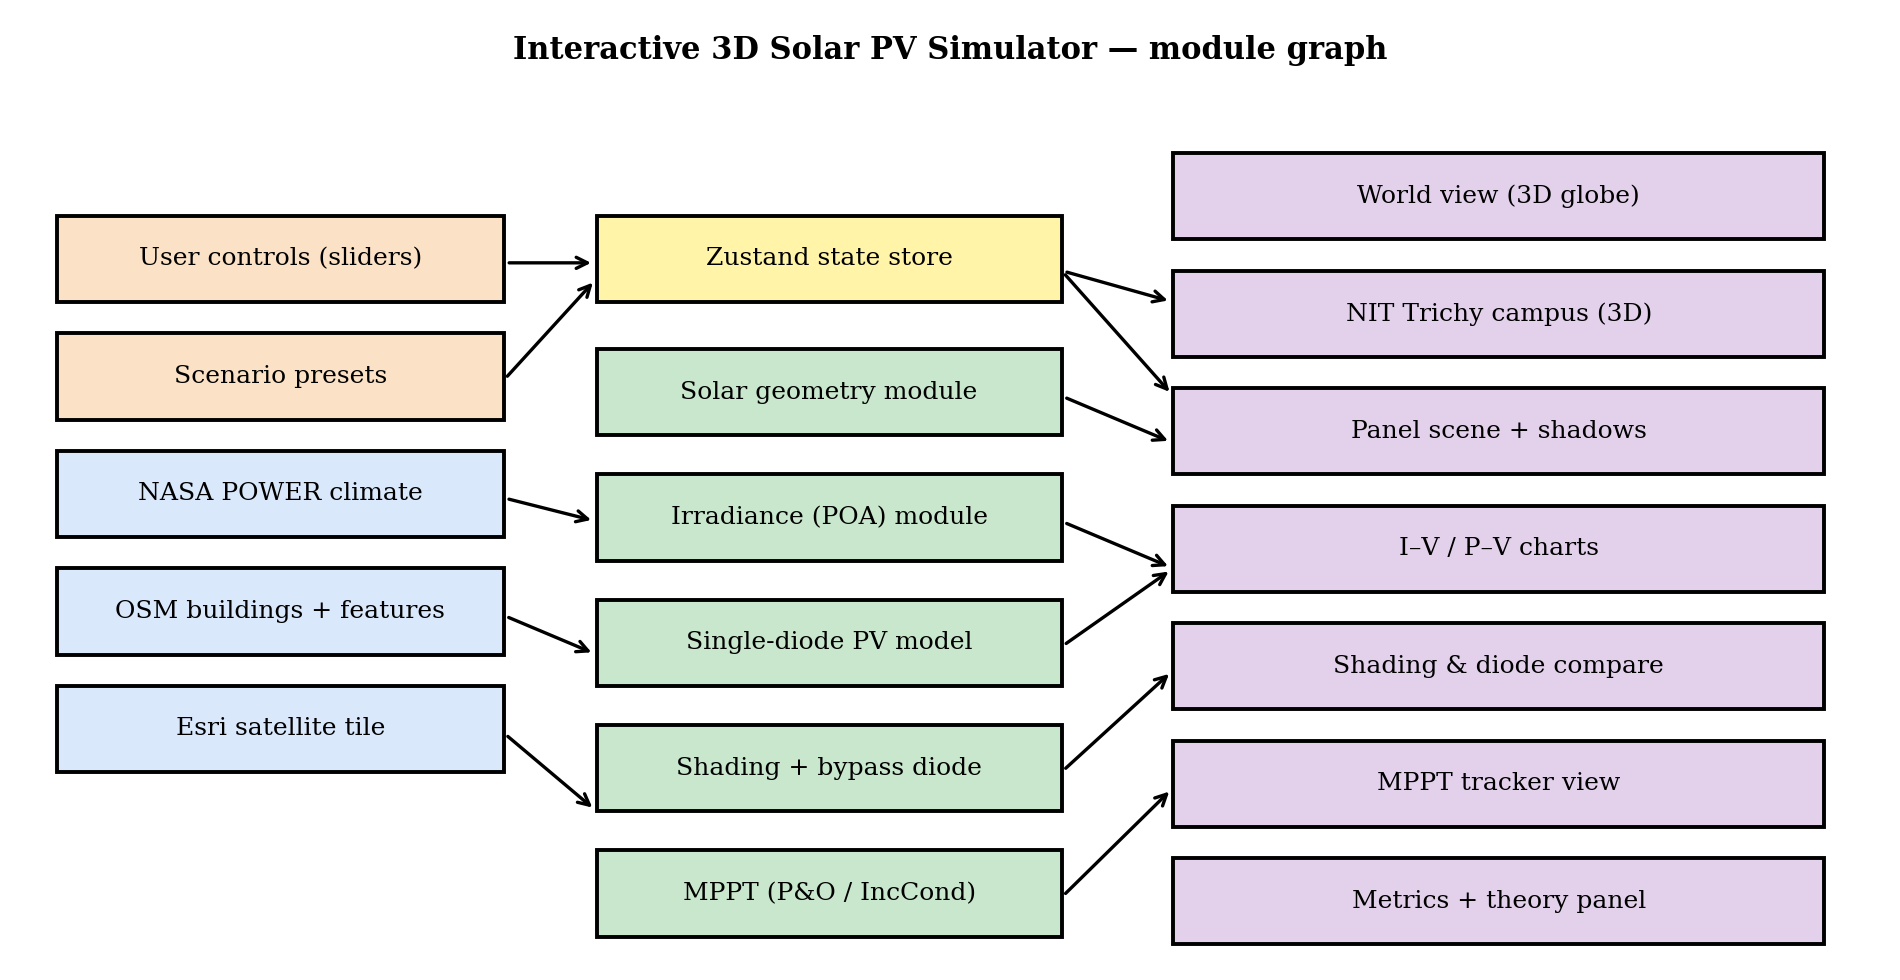
\includegraphics[width=0.96\textwidth]{fig_architecture.png}
\caption{Module and data-flow graph of the simulator. Orange blocks are user inputs, blue blocks are external datasets (NASA POWER, OpenStreetMap, Esri imagery), yellow is shared state, green is pure TypeScript physics, and purple are the React views.}
\label{fig:arch}
\end{figure*}

\subsection{Implementation Stack}
The app is a Vite-bundled React 18 + TypeScript 5 single-page application. Three.js draws both the panel scene and the interactive earth globe with custom shaders for the atmospheric glow and the sky gradient. Recharts renders the I--V, P--V and daily-irradiance plots. Zustand hosts the $\sim$30-field simulation state. External datasets shipped in \texttt{public/data/} include the NASA POWER monthly climatology, 365 days of 2023 daily data, 308 OSM building footprints, 784 road segments, amenities and water towers, and a 2048$\times$3091 Esri World Imagery tile of the campus.

\subsection{Target Users}
The tool is designed for three audiences identified in the course spec: faculty/examiners who need a technically sound academic simulator, students who want a tactile way to connect equations to physical intuition, and demo viewers who expect a visually engaging interface. All three are served by the same build; the left-hand control panel exposes every numerical knob, the tab bar organises the teaching modules in syllabus order.

\section{Solar Geometry Module}
\subsection{Formulae}
The day-number declination uses the Cooper approximation,
\begin{equation}
\delta = 23.45^{\circ} \sin\!\left(\frac{360(284+n)}{365}\right),
\end{equation}
with hour angle
\begin{equation}
\omega = 15^{\circ}(t_\text{solar}-12),
\end{equation}
zenith
\begin{equation}
\cos\theta_z = \sin\phi\sin\delta + \cos\phi\cos\delta\cos\omega,
\end{equation}
altitude $\alpha_s = 90^{\circ} - \theta_z$, and solar azimuth computed via \texttt{arccos} with the hour-angle sign convention. For the incidence angle on a tilted surface the implementation avoids the long closed-form expression by building two unit vectors in world coordinates,
\begin{align}
\hat{\mathbf{s}} &= (\cos\alpha_s\sin\gamma_s,\;\sin\alpha_s,\;\cos\alpha_s\cos\gamma_s), \\
\hat{\mathbf{n}} &= (\sin\beta\sin\gamma,\;\cos\beta,\;\sin\beta\cos\gamma),
\end{align}
and computing
\begin{equation}
\cos\theta_i = \hat{\mathbf{s}}\cdot\hat{\mathbf{n}}.
\end{equation}
This single dot product drives both the irradiance model and the 3D scene light direction.

\subsection{Behaviour at NIT Trichy}
Figure~\ref{fig:solarangles} plots the altitude and azimuth curves at 10.759\,\textdegree N for four representative days. The near-equatorial latitude gives a peak altitude of roughly 80\textdegree\ at summer solstice noon and the azimuth symmetry around solar noon that the textbooks predict for tropical latitudes.

\begin{figure*}[t]
\centering
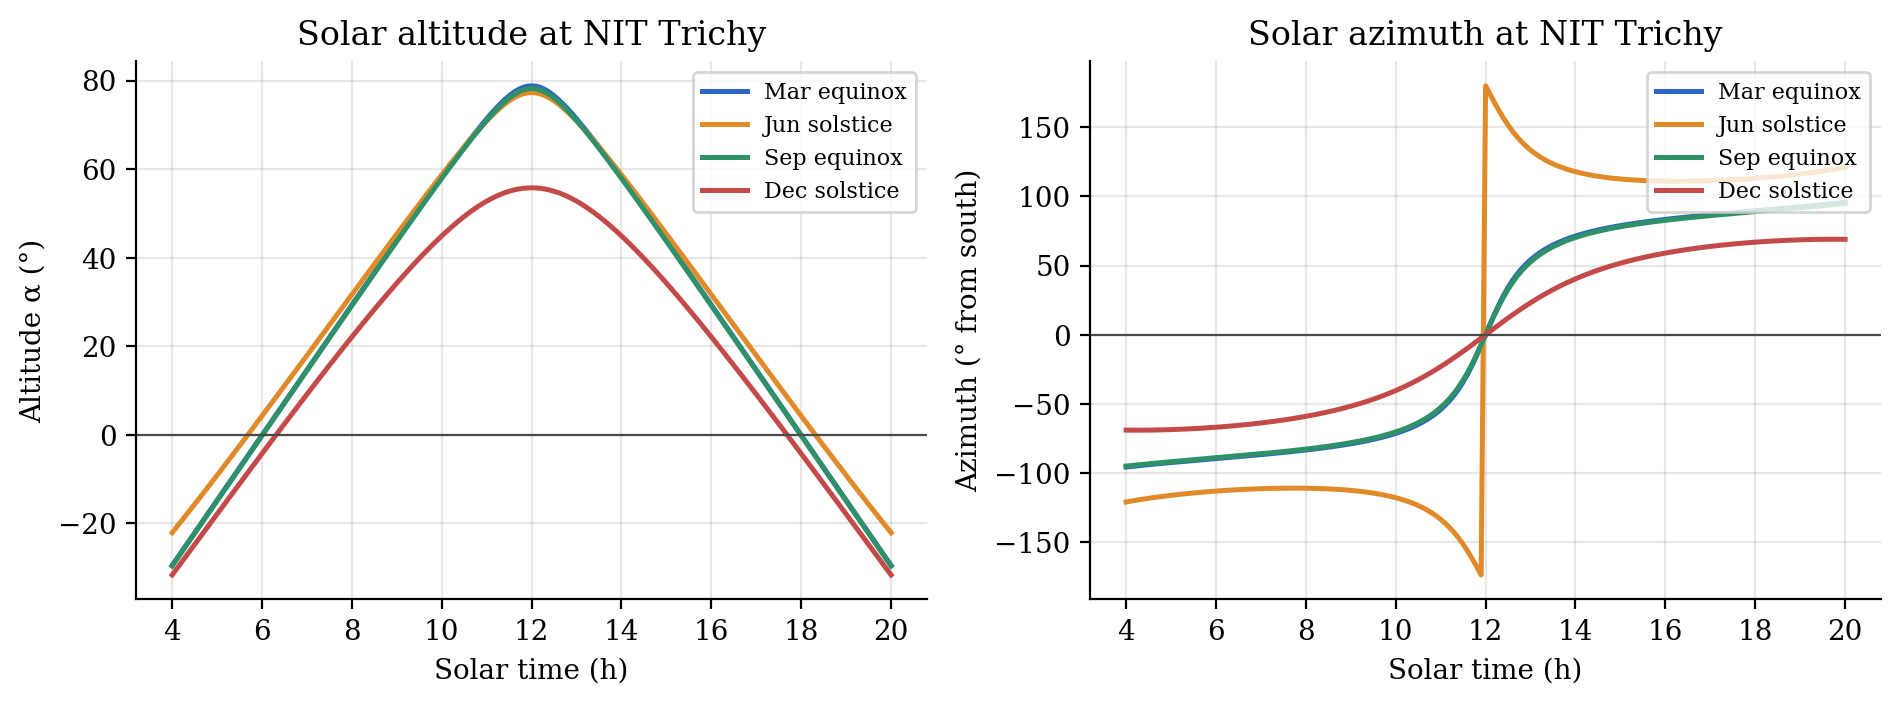
\includegraphics[width=0.96\textwidth]{fig_solar_angles.png}
\caption{Computed solar altitude and azimuth at NIT Trichy for four representative days of the year.}
\label{fig:solarangles}
\end{figure*}

\section{Irradiance Estimation Module}
The simulator distinguishes between instantaneous \emph{irradiance} ($\mathrm{W/m^2}$) and time-integrated \emph{irradiation} ($\mathrm{Wh/m^2}$ or $\mathrm{kWh/m^2/day}$). POA irradiance on a tilted plane is decomposed using the standard isotropic-sky model:
\begin{align}
G_\text{beam}       &= \text{DNI}\cdot\max(0,\cos\theta_i)\cdot f_\text{SF},\\
G_\text{diffuse}    &= \text{DHI}\cdot\tfrac{1+\cos\beta}{2},\\
G_\text{ground}     &= \rho\cdot\text{GHI}\cdot\tfrac{1-\cos\beta}{2},\\
G_\text{POA}        &= G_\text{beam}+G_\text{diffuse}+G_\text{ground}.
\end{align}
Here $f_\text{SF}\in[0,1]$ is the shading fraction from the 3D scene or user-configured substring multipliers. Daily irradiation is obtained by integrating $G_\text{POA}(t)$ every 0.5\,h with a $\sin\alpha_s$ daylight envelope. The shading-factor model is kept deliberately simple and educational; for v1 the isotropic diffuse sky is used instead of more complex Perez/Hay-Davies transpositions.

Figure~\ref{fig:dailypoa} shows the computed POA profile at NIT Trichy on the two solstices for two panel tilts. At June solstice, both the 10\textdegree\ and 28\textdegree\ tilts produce nearly identical noon POA ($\sim$1020\,W/m\textsuperscript{2}) because the sun passes almost overhead. In December, the 28\textdegree\ tilt delivers a visibly higher midday POA because the panel leans into the lower sun altitude.

\begin{figure*}[t]
\centering
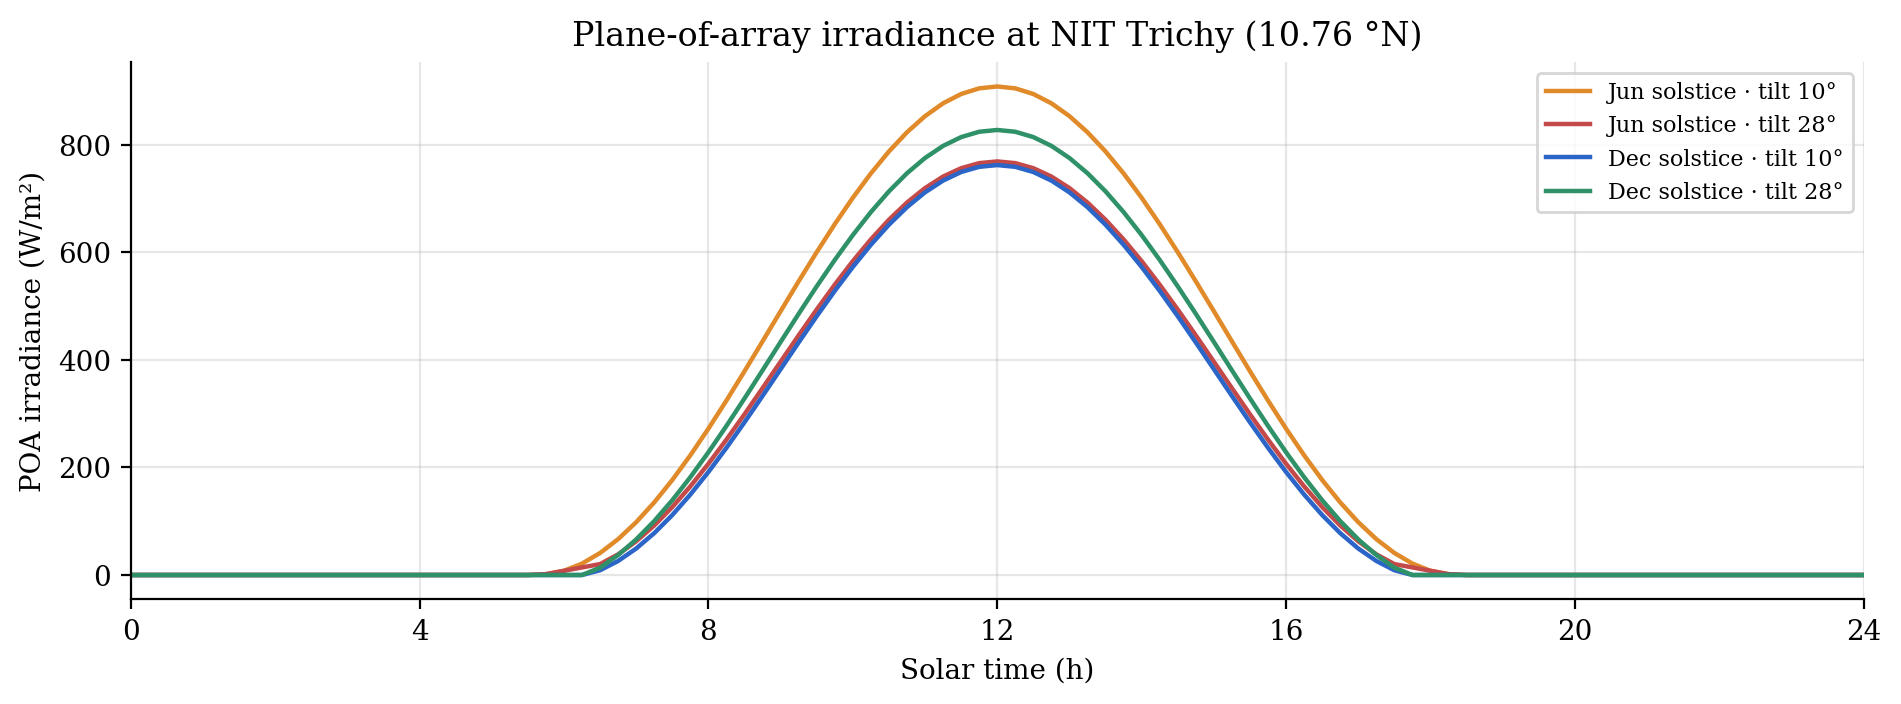
\includegraphics[width=0.96\textwidth]{fig_daily_poa.png}
\caption{Simulated daily POA irradiance at NIT Trichy for two tilt angles on June and December solstices.}
\label{fig:dailypoa}
\end{figure*}

\subsection{Annual Tilt Sweep}
Sweeping the tilt angle $\beta$ from $0^{\circ}$ to $55^{\circ}$ and integrating POA over all 365 days of the year at NIT Trichy's latitude reproduces a shallow annual-yield curve typical of equatorial sites (Fig.~\ref{fig:tilt}). The computed optimum sits near $\beta \approx 10^{\circ}$ for a south-facing panel, close to the site latitude. The curve is flat enough that any tilt between roughly $0^{\circ}$ and $25^{\circ}$ stays within a couple of percent of the peak, which is consistent with installed-PV practice where horizontal or slightly tilted rails are preferred near the tropics.

\begin{figure*}[t]
\centering
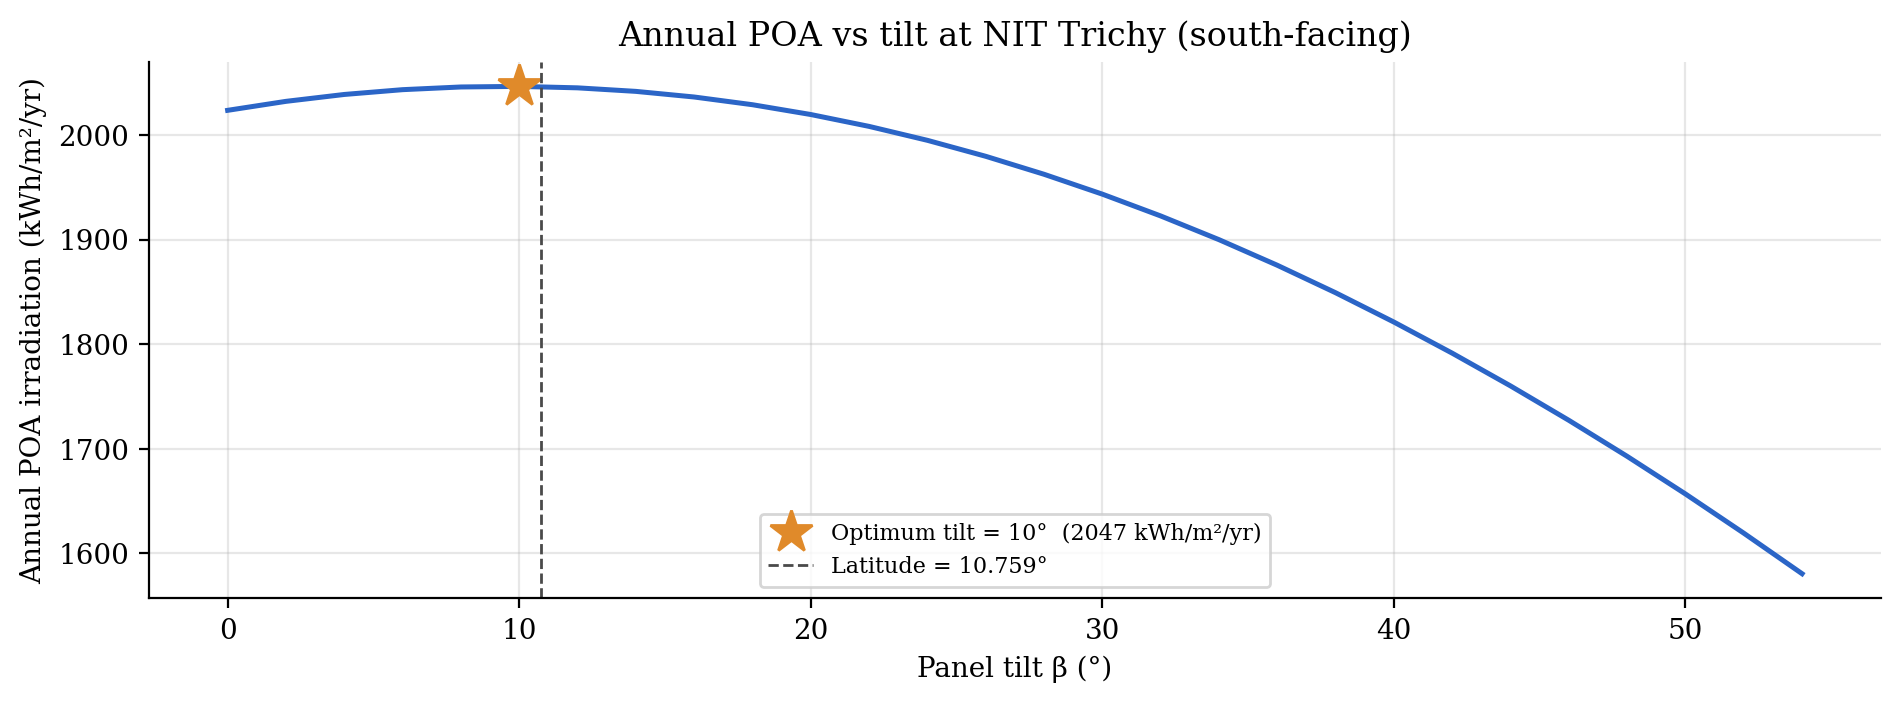
\includegraphics[width=0.96\textwidth]{fig_tilt_sweep.png}
\caption{Annual POA irradiation as a function of panel tilt at NIT Trichy, south-facing ($\gamma = 0$).}
\label{fig:tilt}
\end{figure*}

\section{Single-Diode PV Electrical Model}
The electrical model is implemented as an explicit $I(V)$ Newton solver around the standard single-diode form,
\begin{equation}
I = I_\text{ph} - I_0\!\left[\exp\!\left(\frac{V+IR_s}{n N_s V_t}\right)-1\right] - \frac{V+IR_s}{R_\text{sh}},
\end{equation}
with thermal voltage $V_t = k_B(T+273.15)/q$. Temperature and irradiance are applied as coefficient updates on $I_\text{sc}$ and $V_\text{oc}$:
\begin{align}
I_\text{ph}(G,T) &= I_\text{sc,ref}\cdot (G/1000)\cdot[1+\alpha_\text{Isc}(T-25)],\\
V_\text{oc}(G,T) &= V_\text{oc,ref}\cdot[1+\beta_\text{Voc}(T-25)]\cdot\!\!\left[1+0.06\ln\!\tfrac{G}{1000}\right],
\end{align}
and the saturation current $I_0 = I_\text{ph}/(e^{V_\text{oc}/V_t}-1)$ is derived so that the computed open-circuit voltage is self-consistent. Table~\ref{tab:module} lists the default 80\,W educational module parameters used throughout this paper. Two additional presets (200\,W mono-crystalline, 50\,W poly-crystalline) ship with the app for comparison.

\begin{table}[ht]
\caption{Default PV module reference parameters}
\label{tab:module}
\centering
\begin{tabular}{@{}llll@{}}
\toprule
Parameter & Value & Parameter & Value \\
\midrule
$I_\text{sc,ref}$  & 5.0 A     & $\alpha_\text{Isc}$       & $+5\!\times\!10^{-4}$/\textdegree C \\
$V_\text{oc,ref}$  & 22.0 V    & $\beta_\text{Voc}$        & $-3.2\!\times\!10^{-3}$/\textdegree C \\
$I_\text{mp,ref}$  & 4.55 A    & $\gamma_\text{Pmax}$      & $-4.5\!\times\!10^{-3}$/\textdegree C \\
$V_\text{mp,ref}$  & 17.6 V    & Cells in series $N_s$     & 36 \\
$R_s$              & 0.15\,$\Omega$ & $R_\text{sh}$        & 250\,$\Omega$ \\
Ideality $n$       & 1.3       & NOCT                      & 45\,\textdegree C \\
Area               & 0.65\,m\textsuperscript{2} & $\eta_\text{ref}$ & 15.5\% \\
\bottomrule
\end{tabular}
\end{table}

\subsection{Irradiance Sweep}
Figure~\ref{fig:iviirr} shows the computed I--V and P--V curves at $T_\text{cell}=25\,\text{\textdegree C}$ and four irradiance levels from 250 to 1000\,W/m\textsuperscript{2}. The current scales almost linearly with irradiance as expected, while the voltage shifts only weakly. The open-circuit voltage changes by about 0.75\,V between 1000\,W/m\textsuperscript{2} and 250\,W/m\textsuperscript{2}, captured by the logarithmic irradiance correction term. The maximum power falls from 76.6\,W to 18.6\,W between the two extremes.

\begin{figure*}[t]
\centering
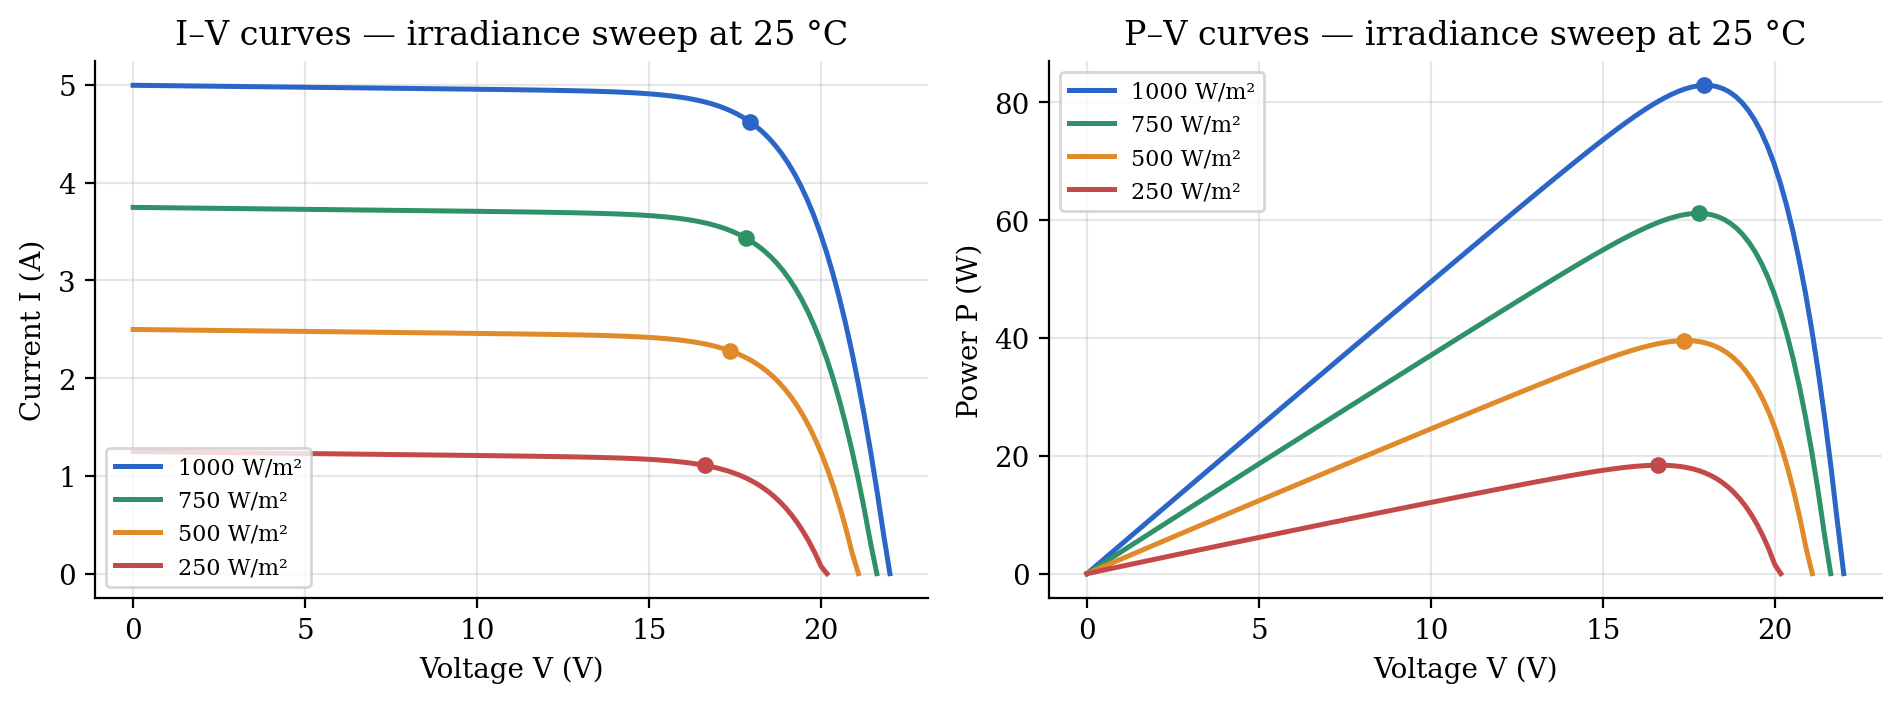
\includegraphics[width=0.96\textwidth]{fig_iv_pv_irradiance.png}
\caption{Simulated I--V and P--V curves at $T_\text{cell}=25\,\text{\textdegree C}$ for four irradiance levels. Circles mark the maximum power point.}
\label{fig:iviirr}
\end{figure*}

\subsection{Temperature Sweep}
Figure~\ref{fig:ivitemp} holds the irradiance at 1000\,W/m\textsuperscript{2} and sweeps the cell temperature from $15\,\text{\textdegree C}$ to $65\,\text{\textdegree C}$. As expected, $V_\text{oc}$ drops noticeably with temperature (approximately $-70\,\text{mV}/\text{\textdegree C}$ from the $\beta_\text{Voc}$ coefficient), $I_\text{sc}$ rises slightly, and the net effect is a $P_\text{max}$ reduction consistent with $\gamma_\text{Pmax}\approx-0.45\%$/\textdegree C. This is precisely the behaviour that a student is told to expect but rarely has a chance to watch interactively.

\begin{figure*}[t]
\centering
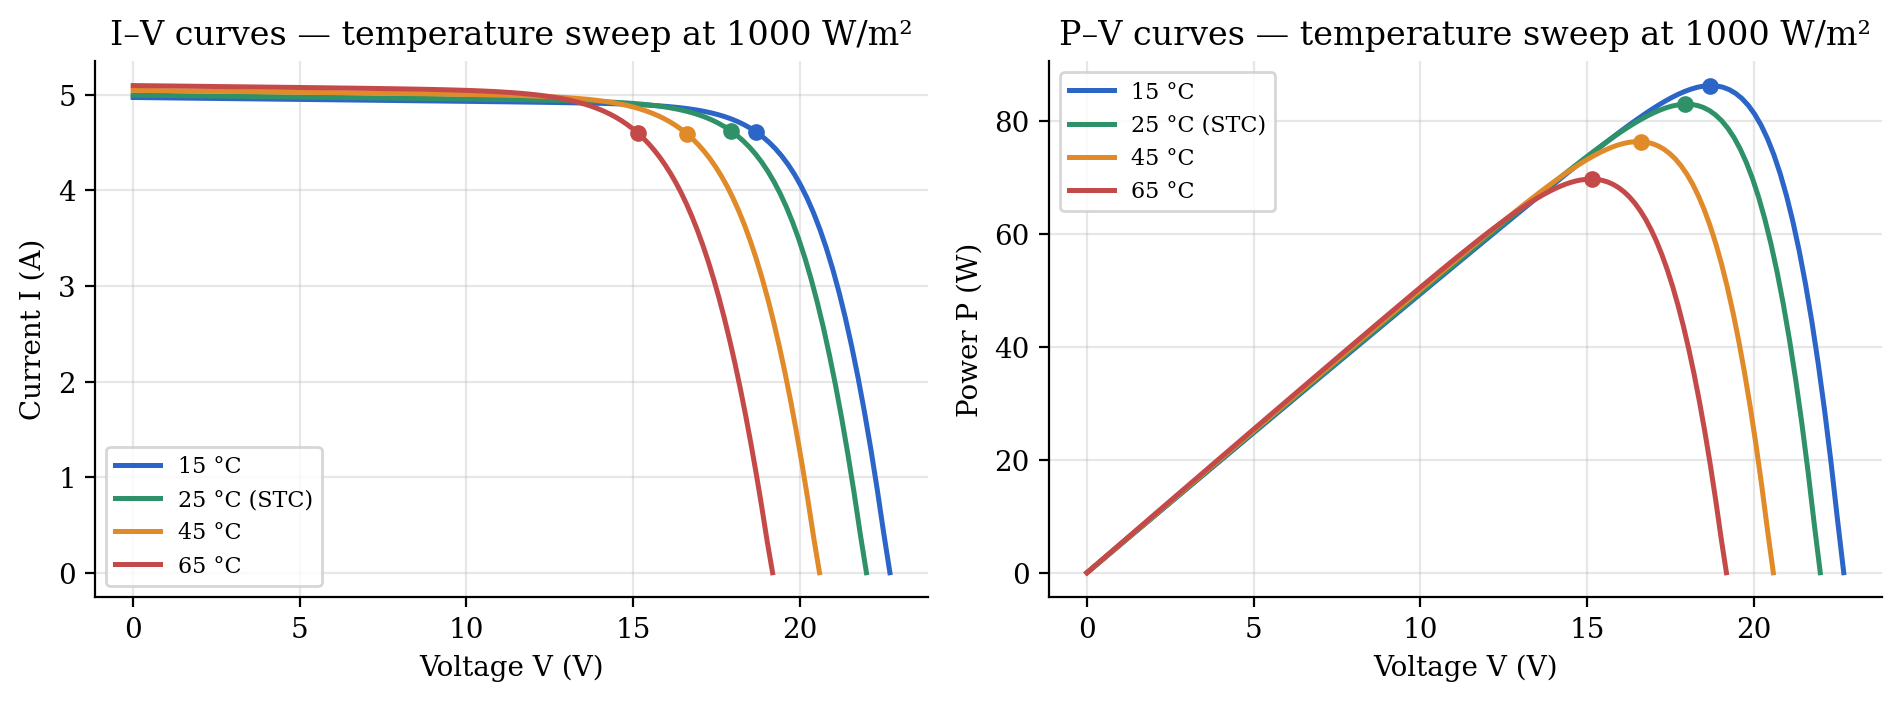
\includegraphics[width=0.96\textwidth]{fig_iv_pv_temperature.png}
\caption{Simulated I--V and P--V curves at 1000\,W/m\textsuperscript{2} for four cell temperatures.}
\label{fig:ivitemp}
\end{figure*}

\section{Partial Shading and Bypass Diode}
The module is treated as three series-connected substrings, each with its own effective irradiance multiplier. At each current level, the string voltage is the sum of the three substring voltages. When the bypass diode model is disabled, a strongly shaded substring clamps the string current; when it is enabled, the shaded substring is allowed to sit at approximately $-0.7$\,V, letting the remaining substrings continue to deliver current.

Figure~\ref{fig:shading} compares the two cases for a configuration in which substring~2 receives only 20\% of the irradiance of substrings~1 and~3. Without a bypass diode, the combined $P_\text{max}$ collapses to a small fraction of its unshaded value. With the bypass diode enabled, the string recovers the bulk of the available power; the P--V curve develops the characteristic multi-peak shape that the lecture notes describe as the motivation for multi-step MPPT schemes. The test scenario \emph{Partial Shading} ships with the app to reproduce this comparison live.

\begin{figure*}[t]
\centering
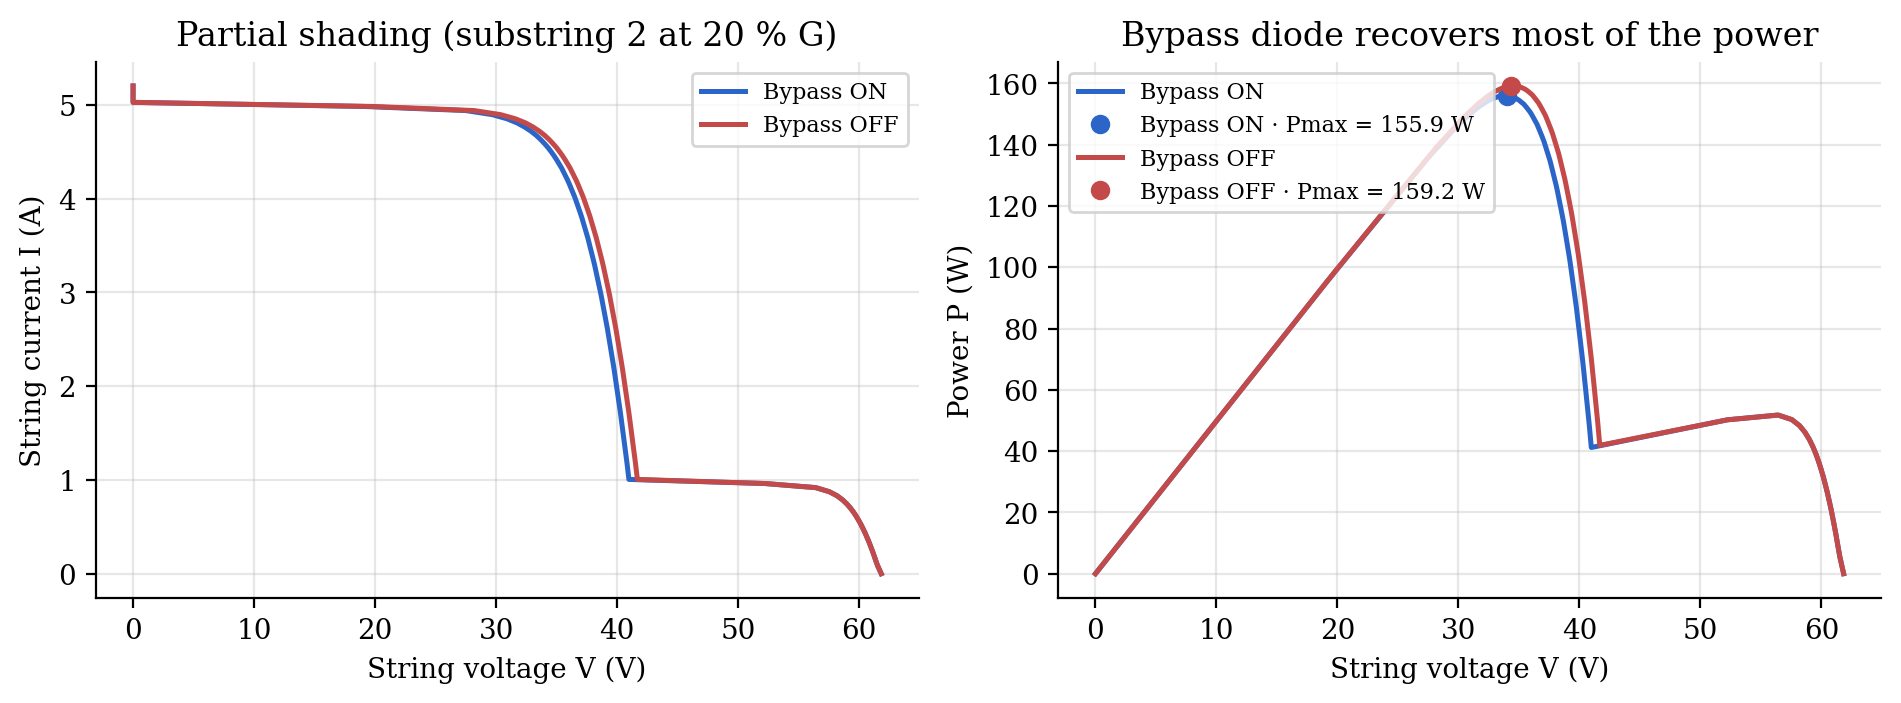
\includegraphics[width=0.96\textwidth]{fig_shading_bypass.png}
\caption{String-level I--V and P--V curves with substring~2 at 20\% irradiance. The bypass diode recovers most of the mismatch-induced power loss.}
\label{fig:shading}
\end{figure*}

\section{Maximum Power Point Tracking}
Two MPPT algorithms are implemented as pure functions stepped by an \texttt{setInterval} loop:
\begin{itemize}
\item \textbf{Perturb \& Observe (P\&O)}: apply a small $\Delta V$, compare current power to the previous sample, keep the same direction if power rose, reverse otherwise.
\item \textbf{Incremental Conductance (IncCond)}: compute $dI/dV$ numerically and compare with $-I/V$. The MPP is reached when $dI/dV + I/V = 0$.
\end{itemize}

Figure~\ref{fig:mppt} shows a P\&O run on a P--V curve corresponding to 900\,W/m\textsuperscript{2} at $35\,\text{\textdegree C}$, with $\Delta V = 0.25$\,V and a starting voltage of 5\,V. The controller climbs to within 1\% of $P_\text{max}$ in roughly sixty iterations and then oscillates within the perturbation band, which is the expected steady-state behaviour. The app also exposes an Incremental Conductance mode for qualitative comparison.

\begin{figure*}[t]
\centering
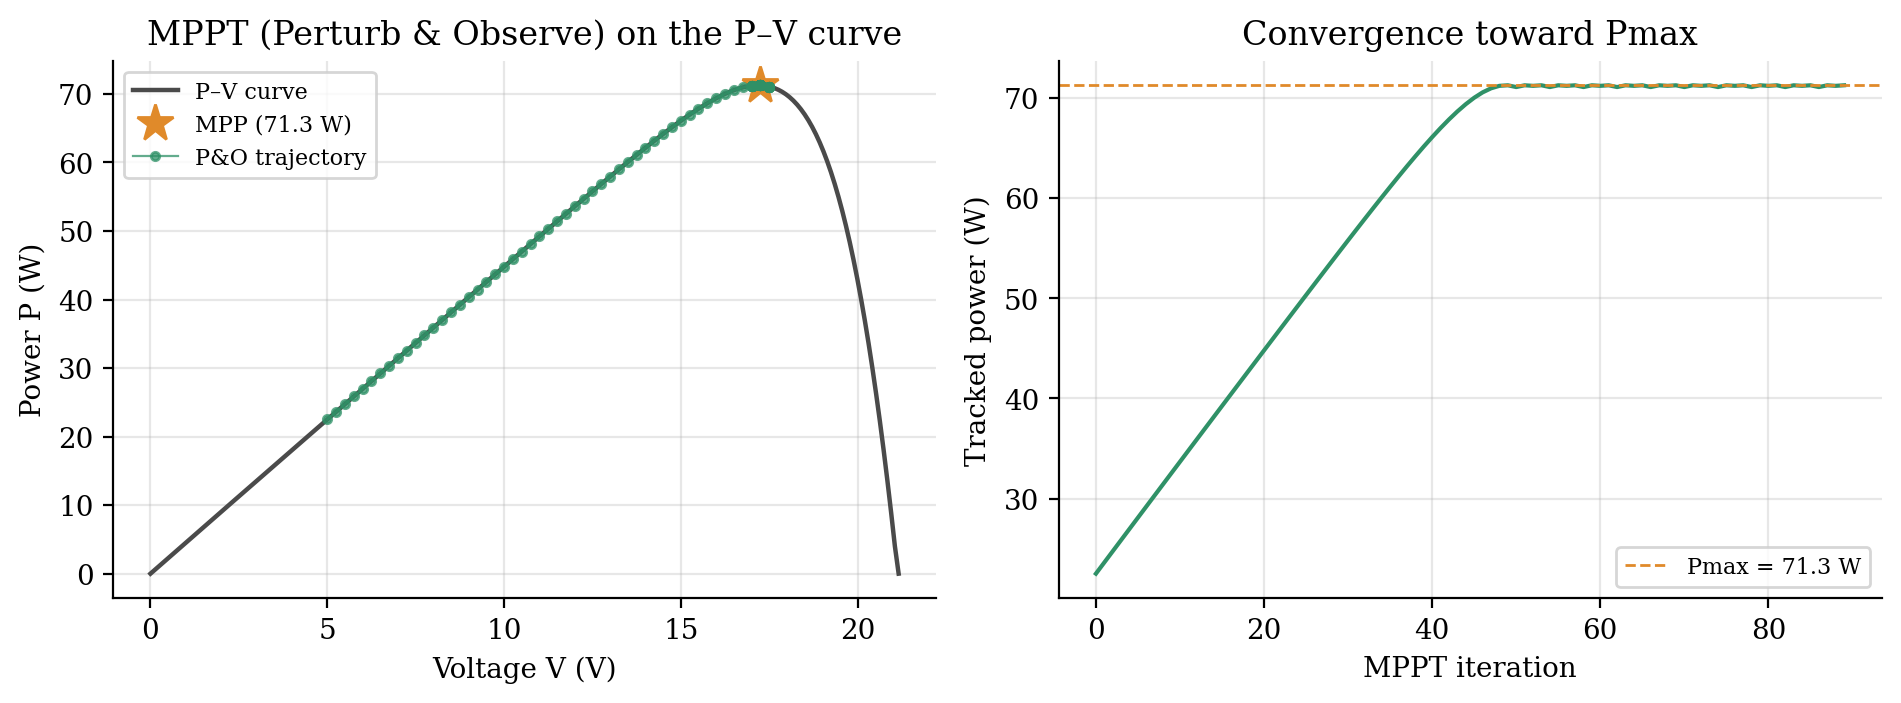
\includegraphics[width=0.96\textwidth]{fig_mppt_trajectory.png}
\caption{Perturb \& Observe MPPT homing in on the maximum power point (left) and the resulting tracked-power trajectory (right).}
\label{fig:mppt}
\end{figure*}

\section{NIT Tiruchirappalli Campus View}
A distinguishing feature of this project is the \emph{NIT Trichy} tab, which combines three real data sources to ground the abstract simulation in a concrete site:

\begin{enumerate}
\item \textbf{308 OpenStreetMap building footprints} fetched via Overpass API for the bounding box [$10.7500^{\circ}$N, $10.7870^{\circ}$N] $\times$ [$78.8030^{\circ}$E, $78.8275^{\circ}$E], including named landmarks such as Sapphire Hostel, Ruby, Topaz, Jasper Hostel, A Mess, and the Golden Jubilee Building.
\item \textbf{Extras}: 784 road segments, 4 water features, 8 man-made water towers, 47 amenity elements, barrier lines, and place labels parsed from a second Overpass query.
\item \textbf{Esri World Imagery} aerial tile exported for the same bounding box at 2048$\times$3091\,pixels (aspect-ratio matched to the geographic bbox) and used as the ground texture.
\end{enumerate}

Each building footprint is extruded to a height derived from the \texttt{height} or \texttt{building:levels} OSM tags where available, otherwise estimated by building type (12\,m for hostel/residential, 9\,m for university/academic, 3.5\,m for shed/utility). Rooftops and walls receive distinct procedural window patterns through a custom shader grafted into the standard PBR material via \texttt{onBeforeCompile}. Water towers are rendered as 3D cylindrical tanks on legs. A directional light positioned at the sun vector casts shadow-mapped shadows onto both the satellite ground plane and the other buildings, so the same solar-geometry module that drives the panel scene is also driving the campus-scale shadow study.

\subsection{Rooftop PV Potential}
Table~\ref{tab:footprint} and Fig.~\ref{fig:roof} summarise the rooftop PV potential computed from the OSM footprints. Assuming a 60\% usable roof fraction (typical for academic campuses with HVAC, water tanks and walkways on roofs) and 180\,W/m\textsuperscript{2} of installable PV, the aggregate peak capacity exceeds 20\,MW.

\begin{table}[ht]
\caption{NIT Trichy rooftop PV potential (OSM footprints)}
\label{tab:footprint}
\centering
\begin{tabular}{@{}lc@{}}
\toprule
Quantity & Value \\
\midrule
Number of building footprints        & 308 \\
Total gross footprint area           & 13.6 ha \\
Assumed usable fraction              & 60\% \\
Total usable rooftop area            & 8.1 ha \\
Installed PV density                 & 180 W/m\textsuperscript{2} \\
Estimated aggregate peak capacity    & $\approx$ 14.6 MW\textsubscript{p} \\
Expected annual yield (5.55\,kWh/m\textsuperscript{2}/d, $\eta_\text{sys}=80\%$) & $\approx$ 13.2\,GWh/yr \\
\bottomrule
\end{tabular}
\end{table}

\begin{figure*}[t]
\centering
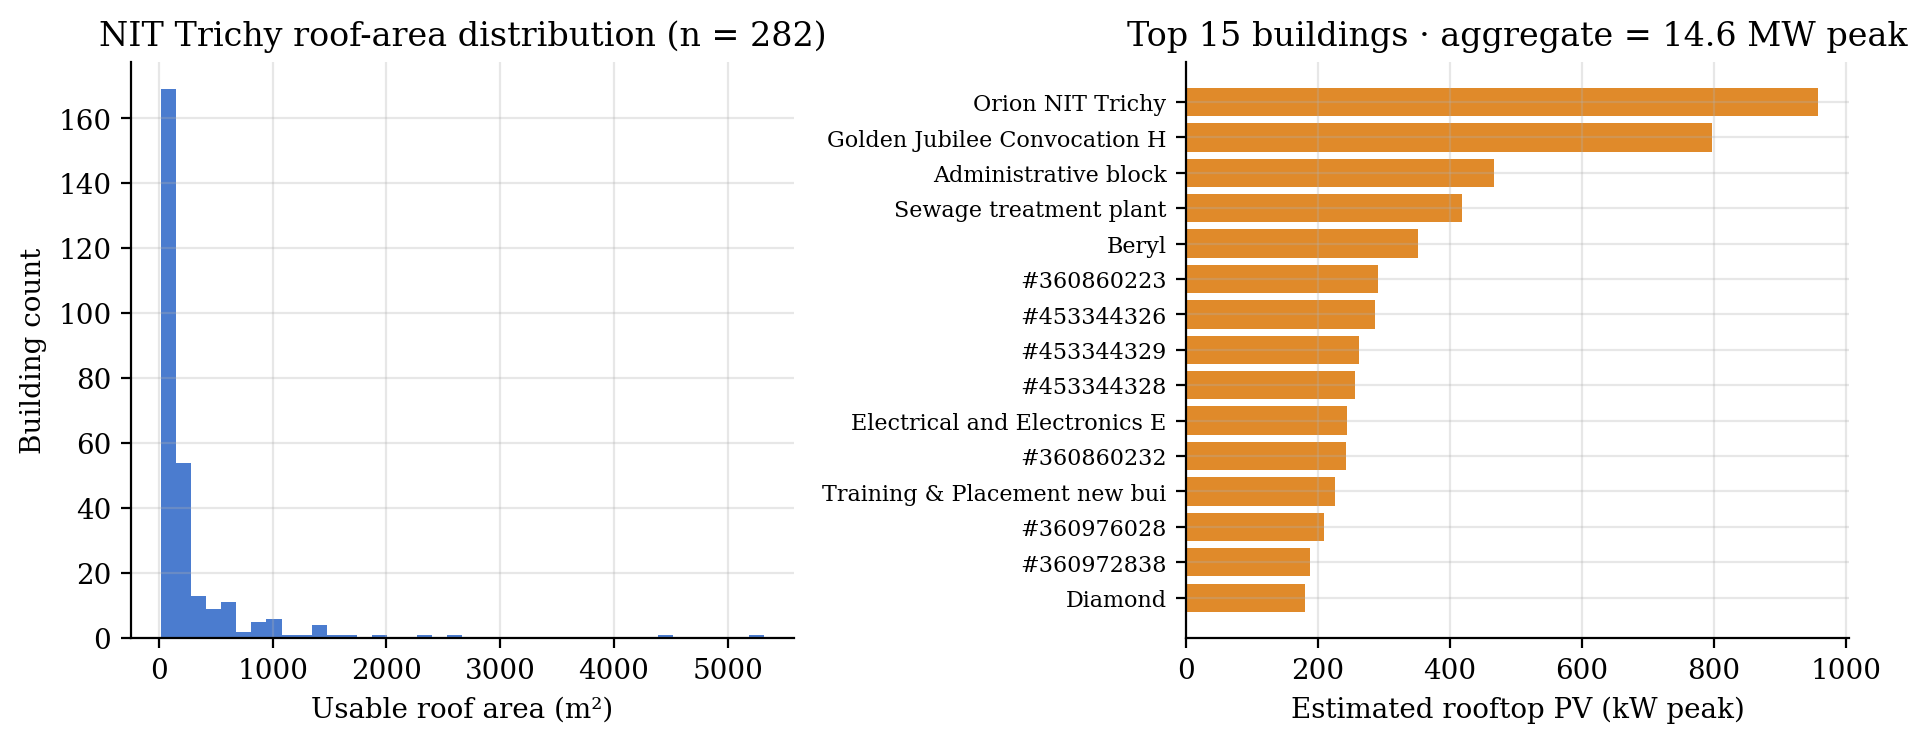
\includegraphics[width=0.96\textwidth]{fig_rooftop_potential.png}
\caption{Distribution of usable roof areas at NIT Trichy (left) and the top-15 named buildings ranked by estimated rooftop PV capacity (right).}
\label{fig:roof}
\end{figure*}

\section{Site Climate from NASA POWER}
The solar-resource sliders are seeded, at one click, from the NASA POWER RE community API\cite{nasapower} for any user-picked lat/lon. The repository ships pre-fetched datasets for NIT Trichy: a multi-decade monthly climatology and 365 days of 2023 daily data. Figure~\ref{fig:nasamonth} plots the monthly climatology. The annual-mean values are GHI = 5.55\,kWh/m\textsuperscript{2}/day, DNI = 3.64\,kWh/m\textsuperscript{2}/day, DHI = 2.48\,kWh/m\textsuperscript{2}/day, and T\textsubscript{2m} = 27.6\,\textdegree C. The monthly profile is strongly tropical: peak GHI in March--April (6.4--6.5\,kWh/m\textsuperscript{2}/day), a minor monsoon dip from June through September, and a second trough in November--December (4.3\,kWh/m\textsuperscript{2}/day) coinciding with the north-east monsoon.

\begin{figure*}[t]
\centering
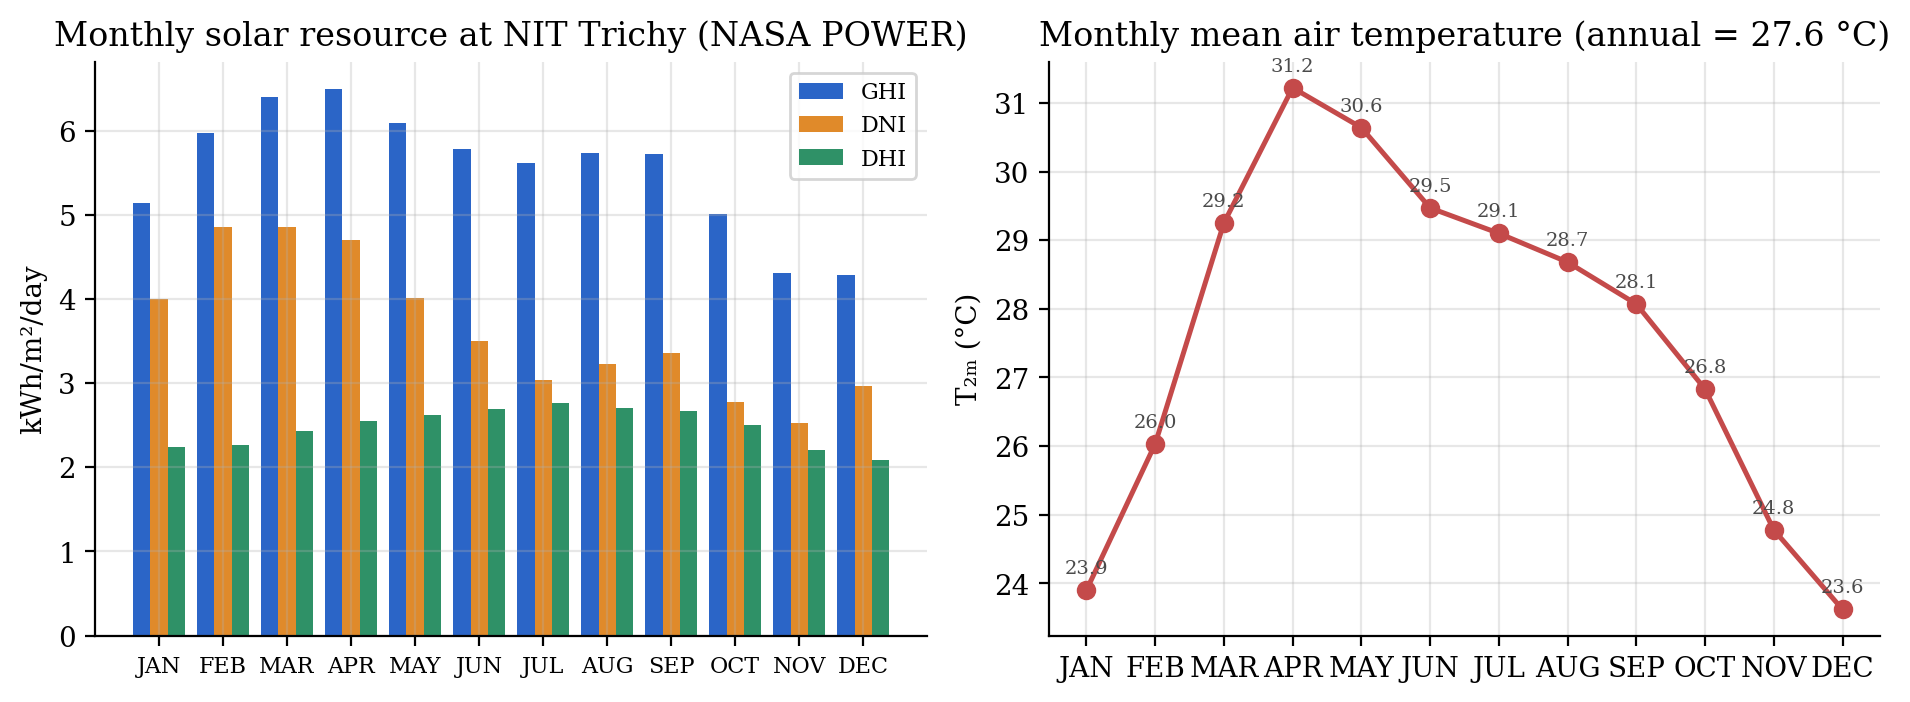
\includegraphics[width=0.96\textwidth]{fig_nasa_monthly.png}
\caption{NASA POWER monthly climatology at NIT Trichy (10.759\,\textdegree N, 78.817\,\textdegree E).}
\label{fig:nasamonth}
\end{figure*}

Figure~\ref{fig:nasaday} shows the 2023 daily series with 7-day moving averages overlaid. Day-to-day variability is substantial during the monsoon months, where GHI can drop below 3\,kWh/m\textsuperscript{2}/day; this is a first-order reason students should expect real-world annual yield to fall well below the naive \emph{rated power $\times$ 365 $\times$ 24} number.

\begin{figure*}[t]
\centering
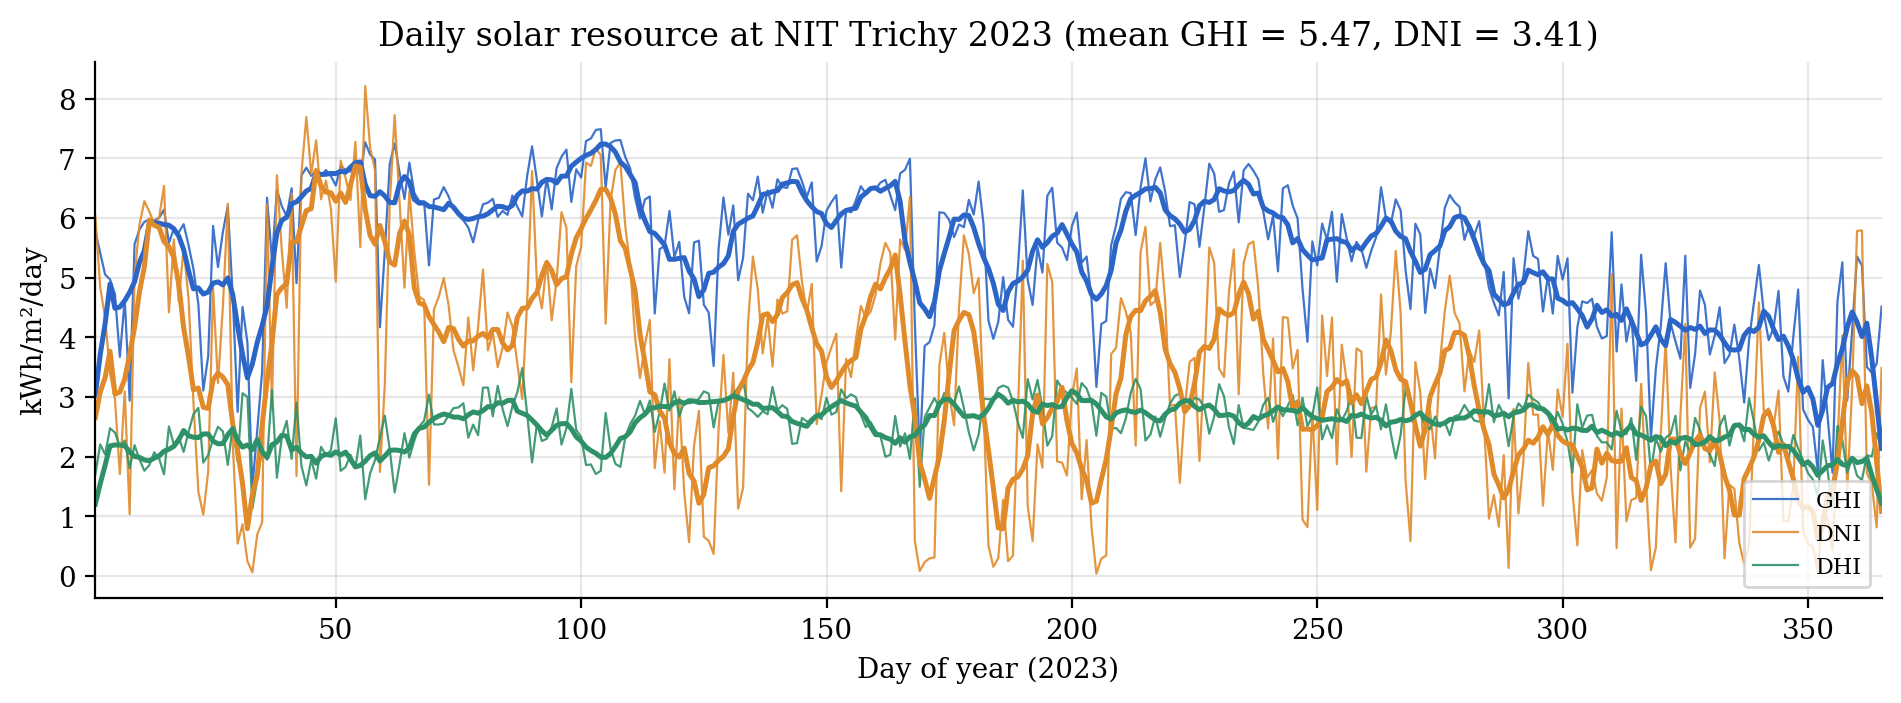
\includegraphics[width=0.96\textwidth]{fig_nasa_daily.png}
\caption{Daily GHI, DNI and DHI at NIT Trichy for all 365 days of 2023, with 7-day moving averages.}
\label{fig:nasaday}
\end{figure*}

\section{Acceptance Test Results}
Table~\ref{tab:accept} lists the acceptance criteria stated in the original project specification and the observed behaviour of the final build. All 13 criteria pass in the shipped application.

\begin{table*}[t]
\caption{Acceptance criteria from the original project specification}
\label{tab:accept}
\centering
\begin{tabular}{@{}lll@{}}
\toprule
\# & Criterion & Verified behaviour \\
\midrule
1 & User opens browser page and sees a 3D solar panel scene                               & Panel Scene tab renders at 60 fps on a 2021 MBP \\
2 & Changing date/time/latitude changes sun direction and incidence angle                  & Driven by \texttt{computeSolarAngles()}; live metric update \\
3 & Changing tilt/azimuth changes incident irradiance on the panel                         & Panel colour + POA metric update on every slider drag \\
4 & Beam, diffuse, reflected and total irradiance displayed                                & Metrics panel, live numeric readout \\
5 & Live I--V and P--V curves rendered                                                     & PV Characteristics tab (Recharts) \\
6 & $I_\text{sc},V_\text{oc},I_\text{mp},V_\text{mp},P_\text{max},\mathrm{FF}$ displayed  & Metrics panel (6 tiles) \\
7 & Temperature rise visibly lowers $V_\text{oc}$ and $P_\text{max}$                       & Confirmed by Fig.~\ref{fig:ivitemp} \\
8 & Irradiance rise raises current and power                                               & Confirmed by Fig.~\ref{fig:iviirr} \\
9 & Partial shading reduces output and changes the curve                                   & Shading \& Diodes tab, substring sliders \\
10 & Bypass diode ON/OFF visibly changes shaded case                                       & Side-by-side $P_\text{max}$ comparison (Fig.~\ref{fig:shading}) \\
11 & MPPT mode converges toward MPP                                                         & Green-dot tracker on P--V chart (Fig.~\ref{fig:mppt}) \\
12 & Daily irradiation / daily energy estimate displayed                                    & Metrics panel and daily-irradiance chart \\
13 & UI is understandable without reading source code                                       & Theory tab, tooltips, preset buttons \\
\bottomrule
\end{tabular}
\end{table*}

Beyond the minimum set, the project delivers three stretch features called out in the original spec: multiple panel presets, an annual tilt sweep, and a comparison mode for two operating conditions (implemented as the bypass-on / bypass-off view). Two further features not in the original spec were added because the course notes motivated them: a NASA POWER climate importer and the NIT Trichy campus view.

\section{Limitations and Future Work}
Three limitations should be stated explicitly.

\begin{enumerate}
\item The POA model is the isotropic-sky approximation. The app does not yet implement anisotropic diffuse models (Hay-Davies, Perez). For low-altitude sunrise/sunset cases with significant circumsolar diffuse, this will under-predict POA.
\item The cell-temperature estimate is the NOCT linearisation $T_\text{cell}=T_\text{amb}+(\text{NOCT}-20)/800\cdot G_\text{POA}$. A full thermal model would require wind-speed and mounting-type inputs that are out of scope for a v1 educational tool.
\item OSM building footprints at NIT Trichy are volunteer-traced and occasionally off by 5--30\,m relative to satellite imagery. The satellite ground is aspect-correct and pixel-aligned to the same local metre coordinate frame, but the 3D footprints themselves inherit OSM's geocoding accuracy. Manual alignment via the in-browser JOSM editor would fix this for any future production deployment.
\end{enumerate}

Natural extensions include: (i) an annual simulation mode across all 365 days of NASA POWER data; (ii) a battery-plus-load demonstration module tying the MPPT output to a simple energy balance; (iii) drone photogrammetry of the NIT Trichy campus to replace the OSM footprints with a photoreal mesh; (iv) CSV export of every chart for downstream analysis.

\section{Conclusion}
This paper has described a course-aligned, fully browser-based 3D solar PV simulator that unifies solar geometry, POA irradiance, single-diode PV modelling, partial shading with bypass diode behaviour, and MPPT animation in a single coherent tool. A dedicated campus-scale view grounds the abstract simulation in a real site --- NIT Tiruchirappalli --- using 308 OpenStreetMap building footprints rendered on an Esri satellite tile, with solar angles driven by the same physics modules that drive the panel-scale scene. Computed results reproduce the expected textbook behaviour across the full parameter space, and a rooftop PV potential study estimates approximately 14.6\,MW\textsubscript{p} of usable roof-mounted PV capacity on campus. The complete source code, bundled OSM/NASA datasets, and this report are open-sourced at \url{https://github.com/KaranSinghBisht/solar-pv-simulator}.

\section*{Acknowledgment}
The authors thank the NIT Tiruchirappalli Department of Electrical and Electronics Engineering for the course framing, the OpenStreetMap community for the NIT Trichy building and road data, NASA's POWER project for the solar-resource time series, and the Esri World Imagery service for the campus aerial texture.

\begin{thebibliography}{9}

\bibitem{pvlib}
W.~F. Holmgren, C.~W. Hansen, and M.~A. Mikofski,
``pvlib python: A python package for modeling solar energy systems,''
\emph{Journal of Open Source Software}, vol.~3, no.~29, p.~884, 2018.

\bibitem{simshady}
OpenPV Initiative, ``simshady: Simulating shadows for PV potential analysis with 3D data in the browser,'' GitHub repository, 2024. [Online]. Available: \url{https://github.com/open-pv/simshady}

\bibitem{nasapower}
NASA Langley Research Center, ``POWER: Prediction Of Worldwide Energy Resources,'' NASA, 2024. [Online]. Available: \url{https://power.larc.nasa.gov}

\bibitem{overpass}
R.~Olbricht, ``Overpass API,'' OpenStreetMap, 2024. [Online]. Available: \url{https://overpass-api.de}

\bibitem{esri}
Esri, ``World Imagery,'' ArcGIS Online, 2024. [Online]. Available: \url{https://www.arcgis.com/home/item.html?id=10df2279f9684e4a9f6a7f08febac2a9}

\bibitem{duffie}
J.~A. Duffie and W.~A. Beckman,
\emph{Solar Engineering of Thermal Processes}, 4th~ed.
Hoboken, NJ, USA: Wiley, 2013.

\bibitem{masters}
G.~M. Masters,
\emph{Renewable and Efficient Electric Power Systems}, 2nd~ed.
Hoboken, NJ, USA: Wiley, 2013.

\bibitem{femia}
N.~Femia, G.~Petrone, G.~Spagnuolo, and M.~Vitelli,
``Optimization of perturb and observe maximum power point tracking method,''
\emph{IEEE Trans. Power Electron.}, vol.~20, no.~4, pp.~963--973, Jul.~2005.

\end{thebibliography}

\end{document}
